\MTtitle{Aprendizaje automático}


%------------------------------------Inteligencia Artificial-------------------------------%
\section{Inteligencia Artificial}

Son muchas las definiciones que se encuentran de la inteligencia artificial o IA, en sus inicios se propone como las  actividades asociadas al pensamiento humano, tareas como, toma de decisiones, resolución de problemas y aprendizaje \citep{CT19}. Con el paso de los años se ha acuñado una definición mas completa: ``la Inteligencia Artificial es una ciencia orientada al diseño y construcción de máquinas que implementen tareas propias de humanos dotados de inteligencia'' \citep{CT1}.\\


Esta ciencia contribuye en el desarrollo de diversos campos de investigación como, Redes neuronales, Computación evolutiva, Algoritmos genéticos, Programación Genética, Teoría del caos. Además tiene un campo amplio de aplicaciones en la sociedad \citep{CT20}, a continuación se muestran algunos ejemplos:

\begin{itemize}

	\item \textbf{Vehículos robóticos}: Un auto robótico sin conductor llamado STANLEY aceleró a través del terreno de Mojave a 22 mph (\textit{miles per hour}, por sus siglas en ingles), terminando el curso de 132 millas primero para ganar el Gran Desafío DARPA 2005

	\item \textbf{Reconocimiento de voz}: Un viajero que llama a \textit{United Airlines} para reservar un vuelo puede tener la conversación completa guiada por un sistema automático de reconocimiento de voz y gestión de diálogos

	\item \textbf{Planificación y programación autónoma}: A cien millones de millas de la Tierra, el programa \textit{Remote Agent} de la NASA se convirtió en el primer programa autónomo de planificación a bordo para controlar la programación de operaciones de una nave espacial

	\item \textbf{Robótica}: \textit{iRobot Corporation} ha vendido más de dos millones de aspiradoras robóticas \textit{Roomba} para uso doméstico

	\item \textbf{Máquina traductora}: Un programa de computadora  traduce automáticamente del árabe al inglés

\end{itemize} 
 

%----------------------Procesamiento de lenguaje natural-------------------------------------%

\section{Procesamiento de lenguaje natural}
\HSection{PROCESAMIENTO DE LN}

El procesamiento de lenguaje natural es una disciplina de la Inteligencia Artificial que se ocupa de la formulación e 
investigación de mecanismos computacionales para la comunicación entre personas y maquinas mediante el uso de Lenguajes 
Naturales.\\

Este campo incluye diferentes técnicas para interpretar el lenguaje humano, que van desde los métodos 
estadísticos y del aprendizaje basado en máquina hasta los enfoques basados en reglas y algorítmicos. Se necesita una amplia variedad 
de métodos porque los datos basados en texto y en voz varían ampliamente, al igual que las aplicaciones prácticas.\\

Dentro de la amplia gama de técnicas para el procesamiento de lenguaje natural, en este trabajo se harán uso de dos de estas técnicas llamadas \textbf{Tokenización} y \textbf{Lematización}. A continuación se describen cada una de ellas junto con un proceso previo llamado pre-procesamiento.\\


%------------------------------------Pre-procesamiento------------------------%

\subsection[Pre-procesamiento]{Pre-procesamiento}


Cuando se recupera  información de la web, se debe limpiar el texto ya que contiene etiquetas definidas por el hipertexto (ver \Tref{cp3:html}{HTML}). Se deben buscar los bloques que brinden información útil para el ámbito de estudio, algunas secciones contienen publicidad o información no relacionada a los datos de interés. Para esto se tiene que realizar un análisis para discriminar la información útil \citep{CD1}. A continuación se muestra un ejemplo de un texto que que requiere ser pre-procesado\\

\begin{mygraybox}[label={box:cp3:texto}]{Texto de ejemplo} 
$<h1>$¡Estudiantes politécnicos apoyan académicamente a alumnos de primaria!$</h1>$\\

$\infty$
$<p>$El Secretario de Educación Pública \Tribar[1][blue][blue!50][blue!20], Esteban Moctezuma Barragán, ha subrayado la importancia \#\#\# de que en la Nueva Escuela Mexicana el Instituto Politécnico Nacional (IPN)\dSmiley, contribuya a fortalecer la educación básica.$</p>$\\
$<!--\ -->$
\end{mygraybox}
\ \\
Como se puede apreciar en el Cuadro \ref{box:cp3:texto} algunas etiquetas requieren ser descartadas para poder obtener únicamente el contenido de la noticias, por ejemplo se debe eliminar el \textit{hipertexto} ( $<h1>$,$</p>$ ) los emojis ( \dSmiley,\Tribar[1][blue][blue!50][blue!20] ) y los símbolos ( $\infty$,\# ). El cuadro \ref{box:cp3:textolimpio} muestra el resultado de limpiar el contenido.\\

\begin{mygraybox}[label={box:cp3:textolimpio}]{Texto limpio} 
¡Estudiantes politécnicos apoyan académicamente a alumnos de primaria!\\

El Secretario de Educación Pública, Esteban Moctezuma Barragán, ha subrayado la importancia  de que en la Nueva Escuela Mexicana el Instituto Politécnico Nacional (IPN), contribuya a fortalecer la educación básica.
\end{mygraybox}
	%\item \textbf{Remover stop-words}: Son pronombres y preposiciones que deben ser removidas para mejorar la compresión del texto.

	%\item  \textbf{Stemming, case-folding, punctuation}: Las palabras que derivan de la misma raíz como hundimiento, se hundió, se reducen a hundir. Una palabra puede tener diferentes significados dependiendo el contexto como la palabra \'Rosa\' puede hacer referencia a una flor o el nombre de una persona, por lo tanto se requiero la heurística del lenguaje específico para poder tomar una decisión en como debe ser interpretada. Los signos de puntuación como el guión medio deben ser tratados con mucho cuidado para realizar una buena tokenización.

%-----------------------------------------Tokenización-------------------------------------%

\subsubsection{Tokenización}

Es el proceso que descompone los textos de una colección en sus unidades mínimas, las palabras
o términos propiamente dichos. A tales elementos se les denomina tokens que conforman una lista de
items que se utilizan para su análisis estadístico, ling{\"u}ístico, de almacenamiento y posteriormente de
recuperación de información. Los tokens a su vez pueden ser identificados mediante una codificación
ASCII o en su defecto UNICODE. De hecho, este proceso permite la identificación de cadenas de caracteres de
forma unívoca, de cara a posteriores tratamientos de depuración, eliminación de signos de puntuación
o la reducción morfológica \citep{CT12}.\\

Continuando con el ejemplo del Cuadro \ref{box:cp3:textolimpio}, se procede a realizar la tokenización del contenido. El Cuadro \ref{box:cp3:tokenizado} muestra el texto dividido en tokens.\\

\begin{mygraybox}[label={box:cp3:tokenizado}]{Texto tokenizado} 
\begin{large}\textbf{¡}\end{large} Estudiantes politécnicos apoyan académicamente a alumnos de primaria \begin{large}\textbf{!}\end{large}\\

El Secretario de Educación Pública \begin{Large}\textbf{,}\end{Large} Esteban Moctezuma Barragán \begin{Large}\textbf{,}\end{Large} ha subrayado la importancia  de que en la Nueva Escuela Mexicana el Instituto Politécnico Nacional \begin{Large}\textbf{(}\end{Large} IPN \begin{Large}\textbf{)}\end{Large} \begin{Large}\textbf{,}\end{Large} contribuya a fortalecer la educación básica \begin{Large}\textbf{.}\end{Large}
\end{mygraybox}
\ \\
Como se puede observar se ha separado por un espacio las palabras, donde cada una representa un token. Ademas los signos de admiración (\begin{large}\textbf{! ¡}\end{large}), los signos de puntuación (\begin{large}\textbf{. ,}\end{large}) y los paréntesis (\begin{large}\textbf{( )}\end{large}), se han divido como tokens independientes.

%-----------------------------------------Lematización-------------------------------------%

\Tlabel{cp3:lematizacion}
\subsubsection{Lematización}

Es el proceso lingüstico que, dada una palabra flexionada se encuentra su
lema. Una palabra flexionada es cuando está en plural, en femenino conjugada,
diminutivo o en superlativo. El lema es la palabra que está en singular para
sustantivo, singular masculino para adjetivo e infinitivo para un verbo \citep{CT13}. Ejemplo:

	\begin{itemize}
		\item amigos, amiga, amiguitos-> Amigo
		\item soy, son, es->Ser
	\end{itemize}

Cabe mencionar que existen diversos grados de lematización:

	\begin{itemize}
		\item Mórfólogica: Es la anteriormente explicada
		\item Sintáctica: Toma en cuenta el contexto donde se encuentra la palabra

	\end{itemize}

En este trabajo se utilizado el grado morfológico. Continuando con el ejemplo tokenizado ( Cuadro \ref{box:cp3:tokenizado} ), El Cuadro \ref{box:cp3:lematizado} muestra el contenido del texto lematizado.\\

\begin{mygraybox}[label={box:cp3:lematizado}]{Texto Lematizado} 
\begin{large}\textbf{¡}\end{large} estudiante politécnicos apoyar academia a alumno de primaria \begin{large}\textbf{!}\end{large}\\

el secretario de educar pública \begin{Large}\textbf{,}\end{Large} esteban moctezuma barragán \begin{Large}\textbf{,}\end{Large} haber subrayar el importar  de que en el nuevo escuela mexicano el instituto politécnico nacional \begin{Large}\textbf{(}\end{Large} ipn \begin{Large}\textbf{)}\end{Large} \begin{Large}\textbf{,}\end{Large} contribuir a fortaleza el educar básico \begin{Large}\textbf{.}\end{Large}
\end{mygraybox}
\ \\



%------------------------------------Apredizje automático-------------------------------%
\section{Aprendizaje Automático}

El Aprendizaje Automático es una rama de la Inteligencia Artificial; permite desarrollar algoritmos que tienen la capacidad de extrapolar (\textit{i.e} predecir) los cambios que se acontecen en una tarea específica \citep{CT2}.\\

El campo utiliza una variedad de algoritmos que aprenden iterativamente de un conjunto de
datos para describir y predecir resultados. A medida en la cual los algoritmos de 
entrenamiento obtienen datos es posible obtener modelos más precisos. Existen cuatro clasificaciones en los métodos \citep{CT21}:

\begin{itemize}

	\item \textbf{Aprendizaje supervisado}: Se proporciona un conjunto de datos de entrenamiento con las respuestas correctas y, con base a este conjunto de 
	entrenamiento, el algoritmo genera un modelo para responder correctamente a todas 
	las entradas posibles

	\item \textbf{Aprendizaje no supervisado}: No se proporcionan datos de entrenamiento, el algoritmo intenta identificar similitudes entre las entradas para clasificar en conjuntos. El enfoque estadístico del aprendizaje no 
	supervisado se conoce como estimación de densidad

	\item \textbf{Aprendizaje reforzado}: Está en algún lugar entre el aprendizaje supervisado y no supervisado. Se indica al algoritmo cuando la respuesta es incorrecta, sin embargo no se informa
	cómo corregirlo. Tiene que explorar y probar diferentes posibilidades hasta que resuelva 
	cómo obtener la respuesta correcta

	\item \textbf{Aprendizaje evolutivo}: La evolución biológica puede verse como un proceso de aprendizaje: los organismos biológicos se adaptan para mejorar sus tasas de supervivencia 
	y la posibilidad de tener descendientes en su entorno. Este comportamiento es modelado, 
	usando un modelo física, el cual corresponde a una puntuación en la 
	solución actual

\end{itemize}

Cabe mencionar que el método implementado en este trabajo es el aprendizaje supervisado, en la sección 3.5 (ver \Tref{cp3:asupervisado}{Aprendizaje supervisado} ) se detalla este enfoque.\\

El aprendizaje automático se puede aplicar a una amplia gama de problemas comerciales, desde la detección de fraudes hasta la orientación al cliente y la recomendación de productos, al monitoreo industrial en tiempo real, el análisis de sentimientos y el diagnóstico médico. Puede asumir problemas que no pueden administrarse manualmente debido a la gran cantidad de datos que deben procesarse \citep{CT22}. Cuando se aplica a grandes conjuntos de datos, a veces puede encontrar relaciones tan sutiles que ninguna cantidad de escrutinio manual las descubriría nunca. Y cuando muchas de estas relaciones ``débiles'' se combinan, se convierten en predictores fuertes.





%------------------------------------Apredizje automático para texto------------------------%

\section{Aprendizaje automático para texto}
\HSection{AA PARA TEXTO}

La extracción de información útil con varios tipos de algoritmos estadísticos es denominado \textbf{Extracción de datos} (\textit{text mining}), \textbf{Analítica de texto} (\textit{text analytics}) o \textbf{Aprendizaje automático para texto} (\textit{Machine learning for text}) \citep{CD1}. En los últimos años este campo ha incrementado por el desarrollo de la web, redes sociales, correos electrónicos, bibliotecas virtuales. Algunas de las aplicaciones son las siguientes:

\begin{itemize}

	\item Etiquetar la web, permite al usuario encontrar paginas de interés

	\item Los proveedores de correos, utilizan la información almacenada para mostrar publicidad de interés al usuario

	\item Algunas páginas ordenan su contenido de acuerdo a su importancia

	\item El análisis de las opiniones es un campo de importancia así como el análisis de sentimientos		

\end{itemize}

El orden de las palabras en un texto brindan un significado semántico el cual no puede ser inferido  solo con la frecuencia de las palabras. Sin embargo, se pueden hacer varias predicciones sin contemplar la semántica. Existen dos tipos de representaciones que son populares:

\begin{itemize}
	\Tlabel{cp3:bolsap}
	\item \textbf{Texto como una bolsa de palabras}: Es la representación mas común. No se contempla el orden de las palabras en el proceso. El conjunto de palabras en el documento se convierten en una representación multidimencional dispersa, el cual corresponde a la dimensión en esta representación. Se utiliza para la clasificación, sistemas de recomendación

	\item \textbf{Texto como un conjunto de secuencias}: En esta representación se extraen sentencias, el orden de las palabras si importa. La unidad son sentencia o párrafos. Es utilizado en aplicaciones que necesitan un fuerte uso de la semántica, esta área se acerca mucho al modelado de lenguaje
\end{itemize}


%----------------------------------Representación del texto--------------------------%
\Tlabel{cp3:representaciont}
\subsection{Representación del texto}

Los métodos de Aprendizaje Automático requieren que la información de la cual aprenderán esté representada en un
formato que facilite su procesamiento. Generalmente esta representación es mediante vectores de valores numéricos. 
Cuando se requiere utilizar estos métodos con información en forma de texto, dicha
información debe ser transformada para generar una representación más adecuada, los métodos mas comunes son: frecuencia, binaria y TF-IDF.\\ 


En este trabajo se utilizarán las dos primeras representaciones basandose en los resultados que han obtenido en el estado del arte. Por lo que sólo se describirán estas dos técnicas junto un ejemplo de su uso.\\


La extracción de características cuenta con dos tareas importantes: formar el vocabulario y crear un vector de características. Para ejemplificar esta tarea observe el Cuadro \ref{box:cp3:corpus} el cual es un corpus de 4 oraciones. Una vez realizado el proceso de extracción de características se obtiene el vocabulario el cual el mostrado en el Cuadro \ref{box:cp3:caracteristicas}.\\\\

\begin{mygraybox}[label={box:cp3:corpus}]{Corpus} 
\begin{equation*}
\begin{bmatrix}
Este&es&el&primer&texto&!!\\
Este&texto&es&el&segundo&texto&???\\
Y&este&es&el&tercero\\
Es&este&el&primer&texto&????\\
\end{bmatrix}
\end{equation*}
\end{mygraybox}

\begin{mygraybox}[label={box:cp3:caracteristicas}]{Vocabulario} 
\begin{equation*}
\begin{bmatrix}
es  & este & el & texto & primer & segundo & tercero & y & ? & !
\end{bmatrix}
\end{equation*}
\end{mygraybox}

Las características son extraídas de 2 formas, binario(donde 1 representa la presencia de la característica y 0 la ausencia) y por frecuencia (donde se cuenta el número de veces que cada característica aparece). Continuando con el ejemplo del Cuadro \ref{box:cp3:corpus} se extraen las características por frecuencia y el resultado se muestra en el Cuadro \ref{box:cp3:frecuencia}, mientras que el Cuadro \ref{box:cp3:binario} muestra las características extraídas de forma binaria.\\


\begin{mygraybox}[label={box:cp3:frecuencia}]{Representación por frecuencia} 
\begin{equation*}
\begin{bmatrix}
1 & 1 & 1 & 1 & 1 & 0 & 0 & 0 & 2\\
1 & 1 & 1 & 2 & 0 & 1 & 0 & 3 & 0\\
1 & 1 & 1 & 0 & 0 & 0 & 1 & 0 & 0\\
1 & 1 & 1 & 1 & 1 & 0 & 0 & 4 & 0\\
\end{bmatrix}
\end{equation*}
\end{mygraybox}

\ \\

\begin{mygraybox}[label={box:cp3:binario}]{Representación binaría} 
\begin{equation*}
\begin{bmatrix}
1 & 1 & 1 & 1 & 1 & 0 & 0 & 0 & 1\\
1 & 1 & 1 & 1 & 0 & 1 & 0 & 1 & 0\\
1 & 1 & 1 & 0 & 0 & 0 & 1 & 0 & 0\\
1 & 1 & 1 & 1 & 1 & 0 & 0 & 1 & 0\\
\end{bmatrix}
\end{equation*}
\end{mygraybox}




%------------------------------------Aprendizaje Supervisado----------------------------------%

\Tlabel{cp3:asupervisado}
\section{Aprendizaje supervisado}
\HSection{A SUPERVISADO}

Los algoritmos de aprendizaje supervisado dependen de datos previamente etiquetado, es decir se necesita un corpus de datos, para llevar acabo el entrenamiento, así 
el algoritmo pueda comprender los datos y con ello determinar que etiqueta debe asignarse a los nuevos datos 
en función del patrón y asociando los patrones a los nuevos datos sin etiquetar. Después de ello, la maquina recibe 
un nuevo conjunto de datos para que el algoritmo de aprendizaje supervisado analice los datos y produzca un resultado 
correcto de los datos etiquetados \citep{CT4}.\\

%------------------------------------Aprendizaje Supervisado----------------------------------%

\Tlabel{cp3:multinomial}
\section{Clasificación multiclase}
\HSection{CLASIFICACIÓN}

Existen dos tipos de clasificaciones: la clasificación binaria, donde se decide si un objetivo pertenece a una clase o no; y la clasificación multiclase en el cual, se tiene un conjunto de datos etiquetados y estos pertenecen a una de $N$ clases diferentes. El objetivo en esta última es construir un algoritmo donde dado otro dato, este pueda predecir de forma correcta la clase a la cual pertenece el nuevo punto. A continuación se describen algunos de los métodos más utilizados de Aprendizaje Automático aplicados a tareas de texto.

%------------------------------------Regresión logistica----------------------------------%

\Tlabel{cp3:regresion}
\subsection{Regresión logística}

La regresión logística es una técnica estadística multivariante que nos permite estimar la relación existente entre una variable dependiente 
no métrica (donde la variable es binaria o también conocida como dicotómica, es decir, solo va a dar como resultado dos alternativas posibles) 
y un conjunto de variables independientes métricas o no métricas \citep{CT6}. Es útil para modelar la probabilidad de un evento ocurriendo como 
función de otros factores. El análisis de regresión logística se enmarca en el conjunto de Modelos Lineales Generalizados que usa como función de 
enlace la función logit. Las probabilidades que describen el posible resultado de un único ensayo se modelan, como una función de variables explicativas, 
utilizando una función logística.\\
% Referencia https://scikit-learn.org/stable/modules/linear_model.html#logistic-regression

Este algoritmo está basado en una regresión lineal, en el cual trata de optimizar la función $l_1$

\begin{equation}
\underset{w,c}{min}{\left|w\right|}_1+C\sum_{i=1}^{n}log(exp(-y_i(X_{i}^{T} w+c ))+1)
\end{equation}

Otra forma de este clasificador es usando la función $l_2$ quien minimiza el costo de la función:

\begin{equation}
\underset{w,c}{min}{\left|w\right|}_1+C\sum_{i=1}^{n}log(exp(-y_i(X_{i}^{T} w+c ))+1)
\end{equation}

La regresión logística es usada extensamente en las ciencias médicas y sociales. Otros nombres para regresión logística usados en varias áreas de 
aplicación incluyen modelo logístico, modelo logit, y clasificador de máxima entropía.

%------------------------------------Naive bayes----------------------------------------%

\Tlabel{cp3:naive}
\subsection{Naive bayes}


\textbf{Naive Bayes} es un conjunto de algoritmos basados en el \textbf{teorema de Bayes} y el uso de la condición \textbf{Naive}. Generalmente utilizan aprendizaje supervisado sobre el conjunto de entrenamiento  $T$ para poder estimar los parámetros 
del modelo generativo, en tanto el conjunto de datos de entrada nuevos se realiza el teorema de Bayes, seleccionando la probable categoría 
que se ha generado \citep{CT7}.\\


Usando la condición \textbf{Naive} todas las características extraídas que utilizan este clasificador se asumen independientes entre sí. La ventaja de usar este clasificador es que 
funciona bien tanto con datos numéricos como con datos textuales y, además, es más fácil de implementar. La desventaja de este clasificador es 
que su rendimiento empeora cuando las características extraídas se correlacionan entre sí.\\

Una derivación de este algoritmo es llamada \textit{Naive Bayes multinomial}, quien permite calcular la probabilidad de pertenencia de un texto $d$ a una clase $c$, como se muestra en la siguiente ecuación:\\

%REF: https://nlp.stanford.edu/IR-book/html/htmledition/naive-bayes-text-classification-1.html
%REF2:https://scikit-learn.org/stable/modules/naive_bayes.html#multinomial-naive-bayes
\begin{equation}
P(c|d) \alpha P(c)\prod_{k=1}^{n}P(t_k|c)
\end{equation}

donde:

\begin{itemize}
	\item $P(c)$ Es la probabilidad de ocurrencia de una clase
	\item $P(t_k|c)$ Es la probabilidad condicional de aparición de una palabra en el conjunto de textos de $c$
	\item $n$ Es el número de palabras en $d$
\end{itemize}


%La forma de estimar $P(c)$ y $P(t_k|c)$ es usando \textit{maximum likelihood estimate}:

\begin{equation}
P(c)=\frac{N_c}{N}
\end{equation}

donde:
\begin{itemize}
	\item $N_c$ Representa la cantidad de características (palabras) de $c$
	\item $N$ Representa la cantidad total de características (es decir la unión de las palabras de cada clase)
\end{itemize}

\begin{equation}
P(t_k|c)=\frac{N_{ck}+\alpha}{N_c+\alpha n}
\label{eq:cp3:naiveBayes}
\end{equation}

donde:
\begin{itemize}
	\item $N_{ck}$=$\sum\nolimits_{k\in T}t_k$ Es el número de veces que la característica $k$ aparece en la clase $c$ del corpus de entrenamiento $T$
	\item $N_c=\sum\nolimits_{k=1}^{n}N_{ck}$ Es el número total de características que contiene la clase $c$
	\item $n$ Es el número de características totales (es decir el vocabulario de la clase $c_1$,$c_2$,$c_3$)
\end{itemize}


Cabe destacar que la complejidad de este algoritmo es $\Theta(mc)$, donde $m$ es el número de características por cada clase $c$.
%----------------------------Maquina de soporte vectorial-------------------------------------%

\Tlabel{cp3:msv}
\subsection{Máquina de soporte vectorial}

Las máquinas de soporte vectorial son sistemas de aprendizaje los
cuales se basan en el uso de un espacio de funciones lineales en un espacio de mayor dimensión inducido
por un kernel, en el que las hipótesis son entrenadas por un algoritmo\citep{CT8}.
Han sido implementadas en clasificación de imágenes, reconocimiento de caracteres, detección de
proteínas, clasificación de patrones, identificación de funciones, etc.
Pertenecen a la categoría de los clasificadores lineales, debido a que inducen separadores lineales
(también conocidos como hiperplanos), ya sea en el espacio original de los ejemplos de entrada, si éstos son separables o cuasi-separables (ruido), o en un espacio transformado (espacio de características),
si los ejemplos no son separables linealmente en el espacio original. La búsqueda del hiperplano
de separación en estos espacios transformados, normalmente de muy alta dimensión, se hará de forma
implícita utilizando las denominadas funciones kernel. Mientras la mayoría de los métodos de aprendizaje
se centran en minimizar los errores cometidos por el modelo generado a partir de los ejemplos
de entrenamiento (error empírico), el sesgo inductivo asociado a la SVM radica en la minimización
del denominado riesgo estructural.
La idea es seleccionar un hiperplano de separación que equidista de los ejemplos más cercanos de
cada clase para, de esta forma, conseguir lo que se denomina un margen máximo a cada lado del hiperplano.
Además, a la hora de definir el hiperplano, sólo se consideran los ejemplos de entrenamiento
de cada clase que caen justo en la frontera de dichos márgenes. 

\Tlabel{cp3:random}
\subsection{Random forest}

Random forest es una combinación de árboles de decisión, de modo que cada árbol depende de los valores de un vector 
aleatorio muestreado independientemente y con la misma distribución para cada uno de estos. Es una modificación sustancial de bagging que construye una 
larga colección de árboles no correlacionados y posteriormente los promedia \citep{CT9}.\\


Bootstrap aggregating (bagging) consiste en obtener muestras aleatorias con reemplazamiento de igual tamaño que el conjunto original\citep{CT24}. Partiendo del conjunto de entrenamiento X= (X1, X2, ...., Xn), mediante la extracción aleatoria con reemplazamiento con el mismo número de elementos que el conjunto original de n elementos, se obtienen B muestras bootstrap Xb= (X1b, X2b, ...., Xnb)
11
donde b=1, 2,.., B. En algunas de estas muestras se habrá eliminado o al menos reducido la presencia de observaciones ruidosas, por lo que el clasificador construido en ese conjunto presentará un mejor comportamiento que el clasificador construido en el conjunto original. Así pues Bagging puede ser útil para construir un mejor clasificador cuando el conjunto de entrenamiento presente observaciones ruidosas.\\

La clasificación es realizada mediante votos, donde un voto se define como, la clasificación regresada por un árbol, la sección con el mayor número de votos es la clasificación asignada a los datos de entrada.



%------------------------------------

\Tlabel{cp3:metricase}
\section{Métricas de evaluación de un modelo de aprendizaje automático}
\HSection{MÉTRICAS}


Una vez generando un modelo de clasificación, es importante medir el desempeño del mismo, con
la intención de mejorar su eficiencia. Una de estas técnicas es la llamada matriz de confusión.\\

\textbf{Matriz de confusión}\\

Una matriz de confusión es una representación de la información de los resultados obtenidos por un
clasificador, dicha matriz suele ser de tamaño n x n, donde n es es el número de clases diferentes con
las que se están trabajando \citep{CT23}.

\begin{figure}[H]
	\centering
	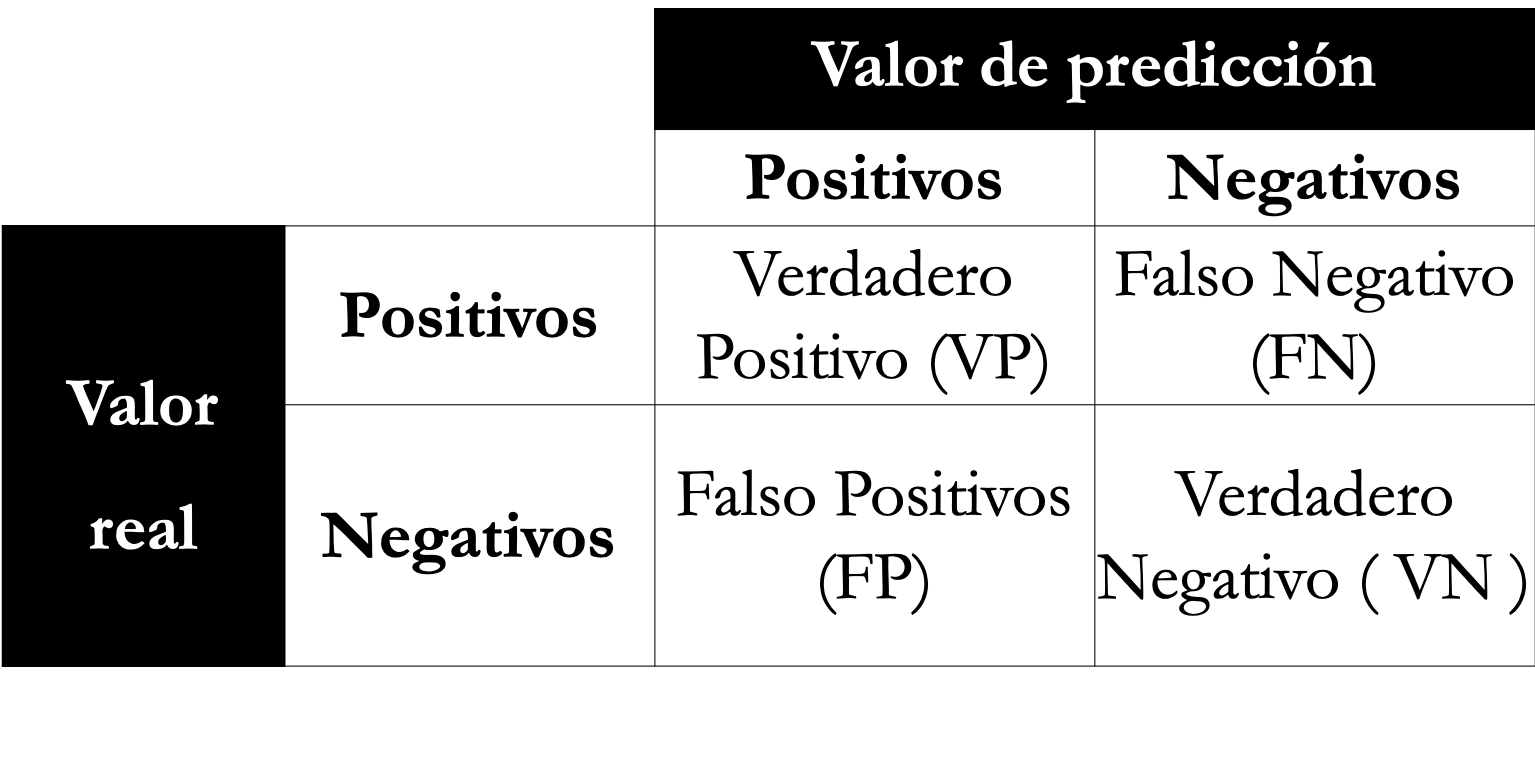
\includegraphics[scale=.3]{imagenes/Capitulo3/MatrizC.png}
	\caption{Matriz de confusión}
	\label{Fig:mconfu}
\end{figure}

La Figura \ref{Fig:mconfu} muestra un ejemplo de matriz de confusión con dos clases, la cual ejemplifica de
manera adecuada las diferentes entradas de la misma, entra las que se encuentran:


\begin{itemize}

	\item \textbf{VP}: Es la cantidad de datos positivos que fueron clasificados correctamente como positivos 
	\item \textbf{FN}: Es la cantidad de datos positivos que fueron clasificados incorrectamente como negativos
	\item \textbf{VN}: Es la cantidad de datos negativos que fueron clasificados correctamente como negativos
	\item \textbf{FP}: Es la cantidad de datos negativos que fueron clasificados incorrectamente como positivos
	
\end{itemize}

La diagonal principal en cualquier matriz de confusión n x n representa el número de predicciones
correctas para cada una de las n secciones.\\

Gracias a la matriz de confusión, es posible obtener ciertas métricas que nos ayudan a evaluar el modelo
de aprendizaje. Entre las que se encuentran:\\


\textbf{Exactitud}: es la proporción del número total de predicciones que son correctas respecto al total.
Se determina utilizando la ecuación:

\begin{equation}\label{eq:1}
	Exactitud = \frac{VP+VN}{VP+VN+FN+FP}
\end{equation}

\textbf{Recall}: Es la proporción de predicciones positivas que fueron correctamente clasificadas. Se determina
utilizando la ecuación:


\begin{equation}\label{eq:2}
	Recall = \frac{VP}{VP+FP}
\end{equation}


\textbf{Precisión}: Es la proporción de predicciones positivas que se clasificaron correctamente. Se determina
con la siguiente ecuación:


\begin{equation}\label{eq:3}
	Precision = \frac{VP}{VP+FN}
\end{equation}


\textbf{F-Measure (F1)}: Se interpreta como la media armónica entre Precisión y Recall. Se determina
con la siguiente ecuación:

\begin{equation}\label{eq:3}
	 F-Measure = 2 \cdot \frac{precision \cdot recall}{precision+recall}
\end{equation}

%------------------------------------

\Tlabel{cp3:validacionc}
\section{Validación cruzada}
\HSection{VALIDACÓN CRUZADA}

El proceso de validación cruzada es uno de los métodos mas usados para generalizar la capacidad de predecir de un modelo clasificador y para prevenir el sobre\-entrenamiento, ademas es usado en la etapa de entrenamiento de un algoritmo de aprendizaje supervisado \citep{CTValidacionC}. Este método consiste en dividir el corpus en $n$ pliegues como se muestra en la Figura \ref{cp3:diagramacv}, cada pliegue está conformado por \textbf{Dobleces} los cuales definen un conjunto de entrenamiento (doblez de color azul cielo) y otro de prueba (doblez de color azul rey). En cada pliegue se entrena el modelo y se prueba, para calcular la exactitud de este conjunto, al terminar el proceso se obtiene el promedio. El objetivo de la validación cruzada es estimar la exactitud del modelo en nuevos datos. Cabe destacar que esta prueba permite encontrar un resultado más robusto y confiable en cuanto a la eficiencia del algoritmo, ya que asegura que los datos no sean manipulados para entrenar y probar con un conjunto de datos a conveniencia (es decir la combinación de información con la exactitud más alta).

%Daniel Berrar, in Encyclopedia of Bioinformatics and Computational Biology, 2019

\begin{figure}[h]
\centering
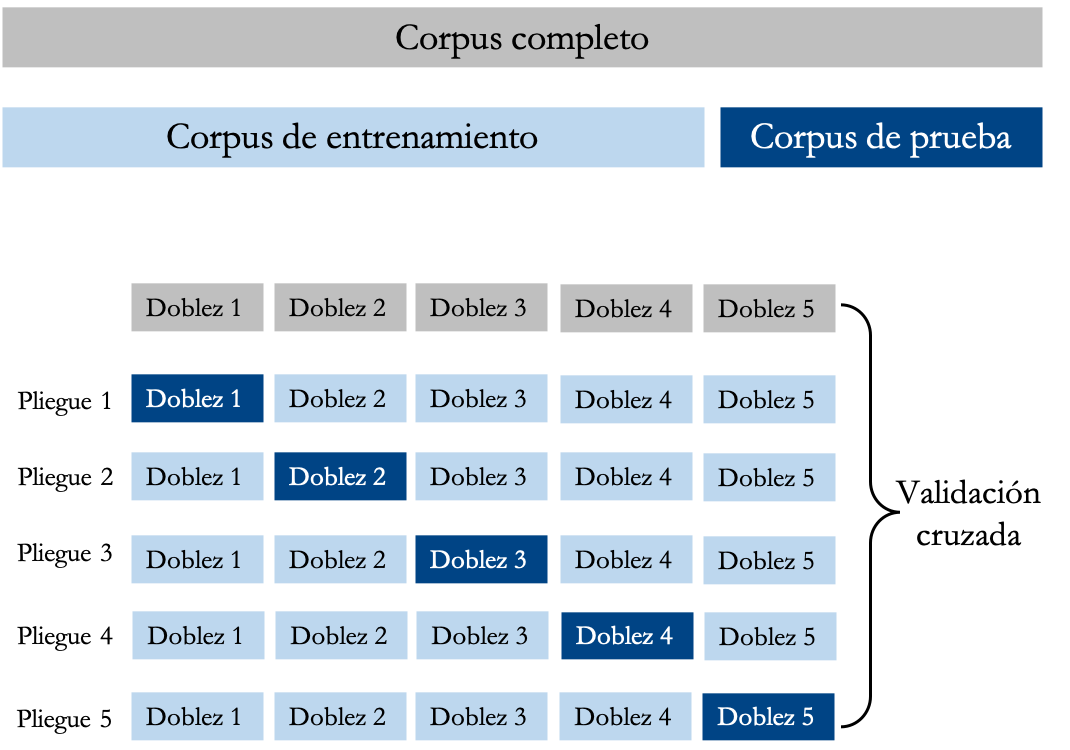
\includegraphics[scale=.55]{imagenes/Capitulo3/validacionc.png}
\caption{Validación cruzada}
\label{cp3:diagramacv}
\end{figure}

